\section{Red neuronal simple (NN-1)}

En primer lugar, se ha implementado una red neuronal simple, compuesta por una capa de entrada y una de salida de tipo softmax.

\subsection{Fundamentos teóricos}

La red neuronal implementada está basada en un modelo de tipo feedforward, que utiliza una arquitectura sencilla con las características descritas a continuación.

Se inicia con una capa de entrada para convertir las imágenes de entrada de forma (28, 28, 1) en vectores unidimensionales de 784 valores, como recomiendan Goodfellow \parencite{goodfellow2016deep} para garantizar compatibilidad con capas densas.

La capa de salida utiliza una activación \textit{softmax}, que convierte los logits en probabilidades interpretables para clasificación multiclase mediante la fórmula:

\[
\sigma(z_i) = \frac{e^{z_i}}{\sum_{j=1}^{K} e^{z_j}}
\]

Esto asegura que las probabilidades sumen 1, facilitando su interpretación como probabilidades \parencite{bishop2006pattern}. La función de pérdida empleada, \texttt{categorical\_crossentropy}, mide la distancia entre las probabilidades predichas y las etiquetas reales usando la fórmula:

\[
H(y, \hat{y}) = -\sum_{i=1}^{K} y_i \log(\hat{y}_i)
\]

Maximizando así la probabilidad de la clase correcta \parencite{murphy2012machine}. Para la optimización, se utiliza Adam \parencite{kingma2014adam}, que combina gradientes adaptativos y momentos para acelerar la convergencia mediante actualizaciones eficientes basadas en primeros y segundos momentos de los gradientes. Finalmente, el aprendizaje supervisado se realiza mediante retropropagación \parencite{rumelhart1986learning} en minibatches, ajustando los pesos para minimizar la pérdida total.


\subsection{Implementación}

En la \autoref{fig:model-red1}, se define una red neuronal secuencial (\texttt{Sequential}) con una capa de entrada \texttt{Flatten}, que aplana las imágenes de tamaño (28, 28, 1) en vectores. Luego, incluye una capa de salida \texttt{Dense} con 10 neuronas y activación \textit{softmax}, adecuada para clasificar en 10 categorías.

El modelo se compila utilizando el optimizador \textit{adam}, la función de pérdida \texttt{categorical \_crossentropy}, y la métrica de precisión (\textit{accuracy}). El entrenamiento se realiza con el método \texttt{fit}, utilizando 10 épocas y un tamaño de batch de 32, mientras se registran métricas como precisión durante el proceso. La salida es configurada con \textit{verbose}=2 para mostrar información detallada en la consola.

\begin{figure}[H]
	\centering
	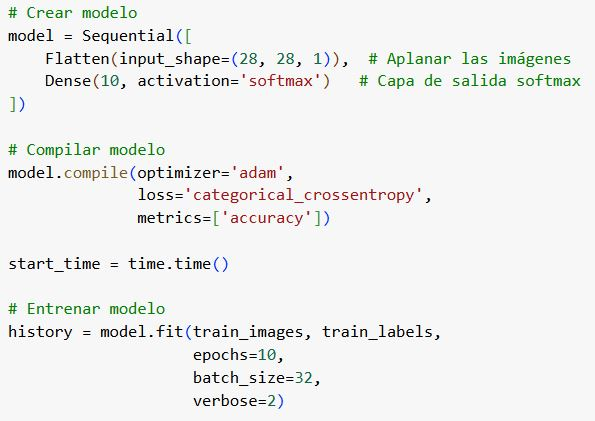
\includegraphics[width=0.7\textwidth]{imgs/model-red1.JPG}
	\caption{Modelado de la primera red neuronal}
	\label{fig:model-red1}
\end{figure}

\subsection{Análisis de resultados}

\begin{figure}[H]
	\centering
	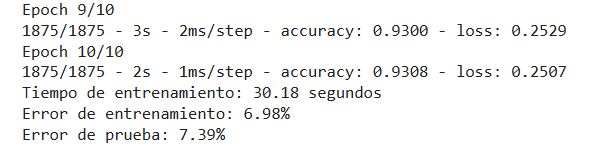
\includegraphics[width=0.7\textwidth]{imgs/results-red1.JPG}
	\caption{Resultados de la primera red neuronal}
	\label{fig:results-red1}
\end{figure}

La primera red neuronal, con una arquitectura simple y sin capas ocultas, logró un error de prueba del 7.39\%, con un tiempo de entrenamiento de solo 30.18 segundos.

Este modelo, aunque básico, ofrece una solución rápida para tareas sencillas de clasificación. Sin embargo, su bajo rendimiento en el conjunto de prueba refleja una capacidad limitada para generalizar, posiblemente debido a su simplicidad y la ausencia de técnicas de regularización o capas intermedias.

\section{Red neuronal multicapa (NN-2)}

En segundo lugar, se ha optado por una red neuronal con una capa oculta de 256 unidades logísticas y una capa de salida de tipo softmax.

\subsection{Fundamentos teóricos}

Esta red tiene una arquitectura algo más compleja que el modelo básico anterior, ya que introduce una capa oculta densa con 256 unidades logísticas y activación \texttt{ReLU} (\textit{Rectified Linear Unit}). La función \texttt{ReLU} está definida como:

\[
f(x) = \max(0, x),
\]

Esta permite manejar de forma eficiente problemas de desvanecimiento del gradiente al solo activar las neuronas con valores positivos, lo que acelera la convergencia del entrenamiento \parencite{nair2010relu}.

Esta capa oculta añade capacidad de representación al modelo, permitiendo aprender características más complejas de los datos de entrada. La capa de entrada y de salida son las mismas definidas en la anterior implementación.


\subsection{Implementación}

La implementación (\autoref{fig:model-red2}) es prácticamente idéntica a la de la red neuronal anterior, salvo por que se le ha añadido entre la capa de entrada y la de salida una capa oculta \texttt{Dense} con 256 neuronas y activación \texttt{ReLU}, que permite aprender características no lineales.

De nuevo, el modelo se compila utilizando el optimizador \textit{adam}, la función de pérdida \texttt{categorical\_crossentropy}, y la métrica de \textit{accuracy}.

El entrenamiento se realiza con el método \texttt{fit}, configurado para 10 épocas, un tamaño de lote de 32, y \textit{verbose}=2 para obtener información del proceso de entrenamiento en consola.

\begin{figure}[H]
	\centering
	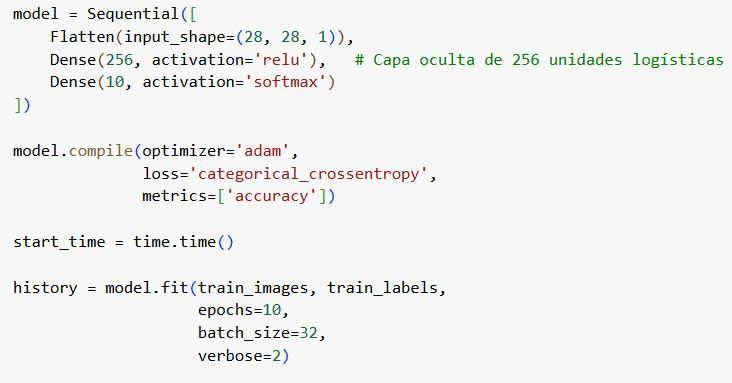
\includegraphics[width=0.7\textwidth]{imgs/model-red2.JPG}
	\caption{Modelado de la segunda red neuronal}
	\label{fig:model-red2}
\end{figure}

\subsection{Análisis de resultados}

\begin{figure}[H]
	\centering
	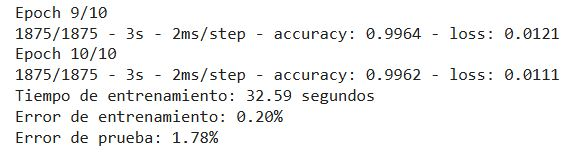
\includegraphics[width=0.7\textwidth]{imgs/results-red2.JPG}
	\caption{Resultados de la segunda red neuronal}
	\label{fig:results-red2}
\end{figure}

La segunda red neuronal introdujo una capa oculta con 256 unidades y activación ReLU, lo que mejoró significativamente su capacidad para aprender características más complejas de los datos.

Esto se tradujo en una mayor precisión y un error de prueba de solo 1.78\%. El tiempo de entrenamiento apenas aumentó con respecto a la anterior y hay una clara mejora en el rendimiento. Comparada con la NN-1, este modelo demuestra cómo una mayor complejidad puede mejorar la generalización en tareas de clasificación.

\newpage
\section{Red neuronal convolucional (NN-3)}

A continuación, se ha considerado una red neuronal convolucional entrenada con gradiente descendente estocástico.

\subsection{Fundamentos teóricos}

La red neuronal implementada corresponde a una red convolucional (CNN), ampliamente utilizada para tareas de clasificación de imágenes debido a su capacidad para capturar patrones espaciales y características jerárquicas en los datos. Este modelo combina capas convolutivas, de \textit{pooling} y densas, cada una diseñada para cumplir una función específica:

\begin{itemize}
	\item \textbf{Capas convolutivas}: las capas \texttt{Conv2D} aplican filtros con tamaño (3, 3) para detectar características locales como bordes y texturas en las imágenes de entrada. Estas capas usan la activación \texttt{ReLU} vista antes, para introducir no linealidad y mejorar la eficiencia computacional \parencite{nair2010relu}.
	\item \textbf{Capas de \textit{Pooling}}: las capas \texttt{MaxPooling2D} con tamaño de ventana (2, 2) reducen la dimensionalidad espacial de las características extraídas, manteniendo la información más relevante y reduciendo la carga computacional. El \textit{max-pooling} selecciona el valor máximo en cada ventana, lo que ayuda a captar las características más prominentes.
	\item \textbf{Capas densas}: la salida de las capas convolutivas es aplanada con \texttt{Flatten} y pasada a una capa completamente conectada (\texttt{Dense}) con 128 neuronas y activación \texttt{ReLU}, para integrar las características aprendidas. Finalmente, una capa de salida con activación \textit{softmax} convierte las predicciones en probabilidades para las 10 clases del problema.
\end{itemize}

El modelo utiliza el optimizador SGD (\textit{Stochastic Gradient Descent}) con tasa de aprendizaje de 0.01 y \textit{momentum} de 0.9. El \textit{momentum} acelera la convergencia al suavizar las actualizaciones de gradiente, evitando oscilaciones en direcciones ortogonales al gradiente principal \parencite{sutskever2013momentum}. La función de pérdida utilizada es \texttt{categorical\_crossentropy}, adecuada para clasificación multiclase, y se valida el rendimiento durante el entrenamiento utilizando un 20\% de los datos de entrenamiento como conjunto de validación interna.

Las CNN, como este modelo, son efectivas para la extracción automática de características espaciales y han demostrado gran éxito en tareas de visión computacional, como describen LeCun \parencite{lecun1998gradient} y Krizhevsky \parencite{krizhevsky2012imagenet}.

\subsection{Implementación}

El modelo secuencial implementado en la \autoref{fig:model-red3} consta de las siguientes capas:
\begin{itemize}
	\item Dos capas convolutivas (\texttt{Conv2D}) con 32 y 64 filtros respectivamente, tamaño de kernel (3, 3) y activación \texttt{ReLU}, para extraer características espaciales locales.
	\item Dos capas de \textit{max-pooling} (\texttt{MaxPooling2D}) con tamaño de ventana (2, 2), para reducir la dimensionalidad espacial.
	\item Una capa de aplanamiento (\texttt{Flatten}) para transformar las características espaciales en un vector.
	\item Una capa densa (\texttt{Dense}) con 128 unidades y activación \texttt{ReLU}, para integrar las características aprendidas.
	\item Una capa de salida (\texttt{Dense}) con 10 unidades y activación \textit{softmax}, para clasificación en 10 clases.
\end{itemize}

El modelo se compila utilizando el optimizador SGD con una tasa de aprendizaje de 0.01 y \textit{momentum} de 0.9. El entrenamiento se realiza con el método \texttt{fit}, configurado para 15 épocas, tamaño de lote de 32 y un \textit{split} del 20\% de los datos de entrenamiento como conjunto de validación. La salida se configura con \texttt{verbose=2} para mostrar el progreso en consola.

\begin{figure}[H]
	\centering
	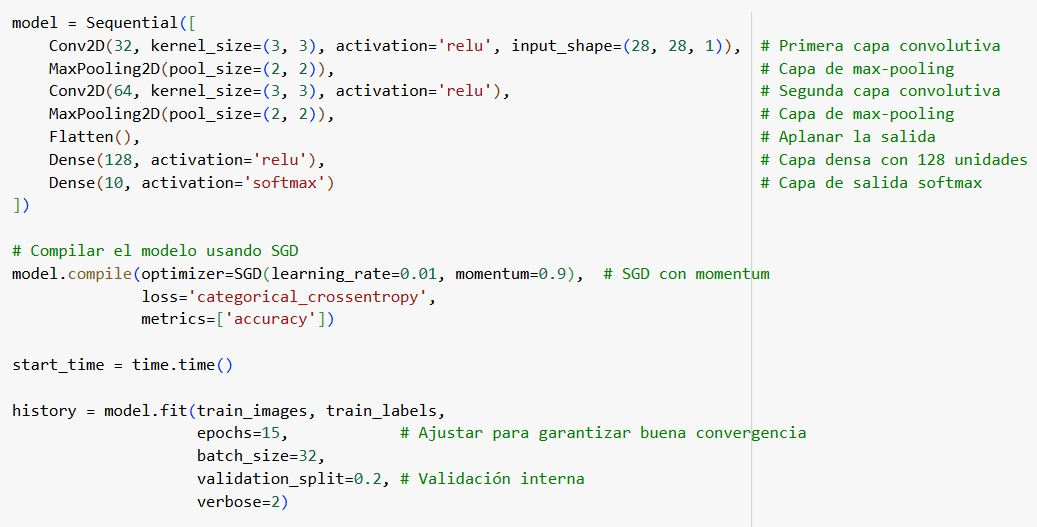
\includegraphics[width=0.7\textwidth]{imgs/model-red3.JPG}
	\caption{Modelado de la tercera red neuronal}
	\label{fig:model-red3}
\end{figure}

\subsection{Análisis de resultados}

\begin{figure}[H]
	\centering
	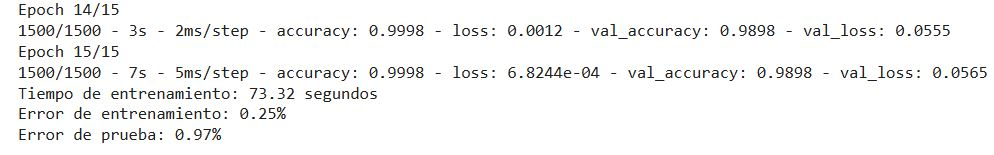
\includegraphics[width=0.7\textwidth]{imgs/results-red3.JPG}
	\caption{Resultados de la tercera red neuronal}
	\label{fig:results-red3}
\end{figure}

La tercera red, una CNN con capas convolutivas y de \textit{pooling}, alcanzó un rendimiento aún mejor, con un error de prueba reducido a 0.97\%.

Este modelo sobresale al extraer características espaciales jerárquicas de las imágenes, lo que lo hace especialmente efectivo para tareas relacionadas con visión computacional. Sin embargo, esto implica un tiempo de entrenamiento mayor en relación con los anteriores, lo que refleja la mayor demanda computacional de este tipo de arquitecturas.

\section{Deep learning con autoencoders (NN-4)}

\textit{Deep learning} usando pre-entrenamiento de autoencoders para extraer características de las imágenes y una red neuronal con capa de salida softmax.

\subsection{Fundamentos teóricos}

Este modelo combina un autoencoder convolucional con una red neuronal supervisada para realizar una clasificación eficiente. El objetivo principal del autoencoder es extraer características relevantes y de menor dimensionalidad a partir de los datos de entrada, las cuales se utilizan posteriormente como entrada para una red neuronal densa para clasificación. Los componentes son los siguientes:

\begin{itemize}
	\item \textbf{Autoencoder convolucional}: este a su vez consta de dos partes:
	\begin{itemize}
		\item \textit{Codificador}: reduce la dimensionalidad espacial de las imágenes utilizando capas convolutivas (\texttt{Conv2D}) con activación \texttt{ReLU} y capas de \textit{max-pooling}. Este proceso permite capturar características jerárquicas de los datos.
		\item \textit{Decodificador}: reconstruye las imágenes originales a partir de las características comprimidas usando capas de \textit{upsampling} y convolución. La última capa utiliza una activación \texttt{sigmoid} para garantizar que las salidas reconstruidas estén en el rango [0, 1], apropiado para imágenes normalizadas \parencite{vincent2010stacked}.
	\end{itemize}
	\item \textbf{Red neuronal supervisada}: las características comprimidas extraídas por el autoencoder son aplanadas y usadas como entrada para una red neuronal densa. Este modelo consta de dos capas densas (\texttt{Dense}), con una capa oculta de 128 unidades y activación \texttt{ReLU}, y una capa de salida con activación \texttt{softmax} para clasificación multiclase.
	\item \textbf{Optimización}: el autoencoder se entrena usando el optimizador \textit{adam}, que ajusta los pesos para minimizar la pérdida \texttt{binary\_crossentropy}, adecuada para tareas de reconstrucción. Posteriormente, la red supervisada se entrena con el optimizador SGD y \textit{momentum}, para mejorar la convergencia y evitar oscilaciones.
	\item \textbf{Entrenamiento supervisado tras la extracción de características}: las características comprimidas actúan como un conjunto de datos transformado con información relevante, lo que reduce la complejidad del modelo supervisado y mejora su capacidad de generalización \parencite{hinton2006reducing}.
\end{itemize}

\subsection{Implementación}

El código consta de tres partes principales:
\begin{enumerate}
	\item \textbf{Definición del autoencoder}:
	\begin{itemize}
		\item Se utiliza \texttt{Input} para definir la forma de entrada (28, 28, 1).
		\item El codificador tiene dos capas convolutivas (\texttt{Conv2D}) con 32 y 64 filtros, seguidas de capas de \textit{max-pooling} (\texttt{MaxPooling2D}). La activación es \texttt{ReLU} y el \texttt{padding} es \texttt{'same'} para preservar dimensiones.
		\item El decodificador invierte el proceso mediante capas de \textit{upsampling} (\texttt{UpSampling2D}) y convoluciones para reconstruir la entrada original.
		\item El modelo es compilado con el optimizador \textit{adam} y pérdida \texttt{binary\_crossentropy}.
	\end{itemize}
	
	\begin{figure}[H]
		\centering
		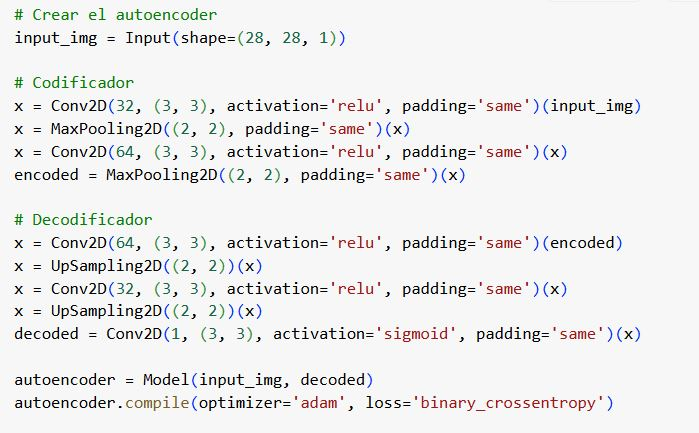
\includegraphics[width=0.7\textwidth]{imgs/model-1-red4.JPG}
		\caption{Modelado de la cuarta red neuronal (pt. 1)}
		\label{fig:model-1-red4}
	\end{figure}
	
	\item \textbf{Entrenamiento del autoencoder}:
	\begin{itemize}
		\item Se entrena el autoencoder usando \texttt{fit} con los datos de entrenamiento tanto como entrada como salida, durante 10 épocas, con un tamaño de lote de 256 y validación del 20\%.
		\item Una vez entrenado, el codificador es extraído y utilizado para transformar los datos en representaciones comprimidas.
	\end{itemize}
	
	\begin{figure}[H]
		\centering
		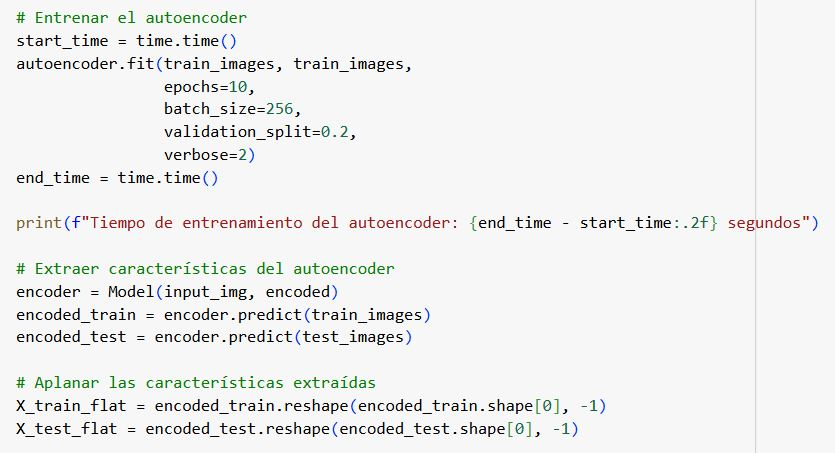
\includegraphics[width=0.7\textwidth]{imgs/model-2-red4.JPG}
		\caption{Modelado de la cuarta red neuronal (pt. 2)}
		\label{fig:model-2-red4}
	\end{figure}
	
	\item \textbf{Red supervisada para clasificación}:
	\begin{itemize}
		\item La red neuronal supervisada tiene una capa densa oculta con 128 neuronas y activación \texttt{ReLU}, seguida de una capa de salida con 10 neuronas y activación \texttt{softmax}.
		\item Se entrena utilizando \texttt{SGD} con tasa de aprendizaje 0.01 y \textit{momentum} de 0.9, minimizando la pérdida \texttt{categorical\_crossentropy}.
		\item El entrenamiento se realiza durante 20 épocas, con un tamaño de lote de 32 y validación del 20\%.
	\end{itemize}
	
	\begin{figure}[H]
		\centering
		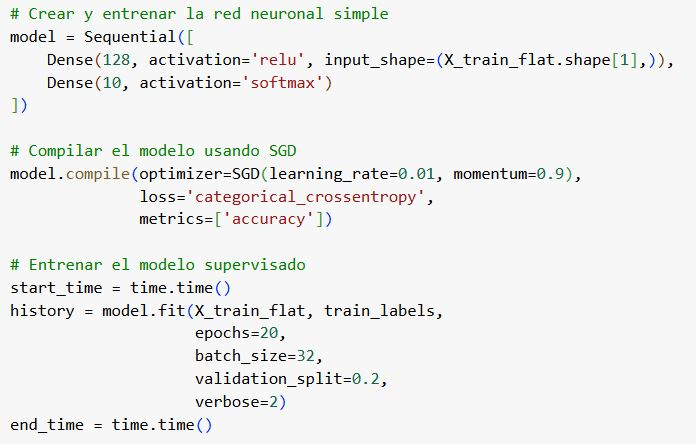
\includegraphics[width=0.7\textwidth]{imgs/model-3-red4.JPG}
		\caption{Modelado de la cuarta red neuronal (pt. 3)}
		\label{fig:model-3-red4}
	\end{figure}
\end{enumerate}

\subsection{Análisis de resultados}

\begin{figure}[H]
	\centering
	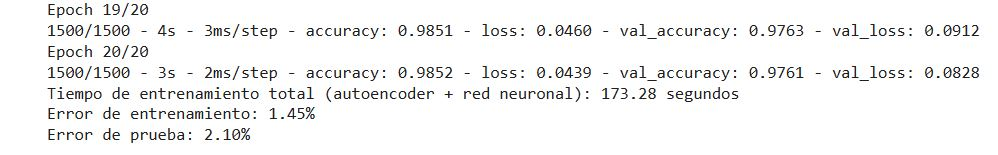
\includegraphics[width=0.7\textwidth]{imgs/results-red4.JPG}
	\caption{Resultados de la cuarta red neuronal}
	\label{fig:results-red4}
\end{figure}

El cuarto modelo, que combina un autoencoder con una red supervisada, logró un error de prueba de 2.10\%. Aunque no alcanzó el rendimiento de la NN-3 (la CNN) en términos de precisión, este modelo es útil para tareas que requieren una reducción de dimensionalidad previa, como la compresión de datos o la extracción de características relevantes, además requiere menos tiempo que el modelo anterior al utilizar una red neuronal más simple.


\section{Red neuronal convolucional mejorada (NN-5)}

A continuación, se ha intentado combinar algunas de las técnicas anteriores para implementar una red neuronal que se acerque lo máximo posible a una \textit{accuracy} de 99.7\%.

\subsection{Fundamentos teóricos}

Este modelo mejorado combina técnicas avanzadas de deep learning para optimizar la clasificación de imágenes. La arquitectura se basa en redes convolucionales (CNN), a las que se integran estrategias de regularización, aumento de datos y optimización, detalladas a continuación:

\begin{itemize}
	\item \textbf{Aumento de datos}: se utiliza \texttt{ImageDataGenerator} para aplicar transformaciones como rotación, desplazamientos horizontales y verticales, y zoom. Estas técnicas aumentan artificialmente el tamaño del conjunto de datos, ayudando a prevenir el sobreajuste y mejorando la generalización del modelo.
	\item \textbf{Arquitectura del modelo}: la red incluye capas convolutivas (\texttt{Conv2D}) y de \textit{max-pooling}, que extraen y reducen las características espaciales. Cada capa convolutiva está seguida de una capa de \textit{dropout}, que aleatoriamente apaga un porcentaje de neuronas durante el entrenamiento para reducir el sobreajuste \parencite{srivastava2014dropout}. Las capas densas al final permiten integrar características y realizar la clasificación final.
	\item \textbf{Regularización con \textit{Dropout}}: las capas \texttt{Dropout} con tasas de 25\% y 50\% reducen el riesgo de sobreajuste al evitar que el modelo dependa excesivamente de características específicas. Esto mejora la capacidad del modelo para generalizar a datos no vistos \parencite{srivastava2014dropout}.
	\item \textbf{Optimización avanzada}: el optimizador \textit{adam} se utiliza con una tasa de aprendizaje inicial de 0.001, combinando la eficiencia de SGD con el cálculo de momentos adaptativos. La pérdida \texttt{categorical\_crossentropy} mide la distancia entre las etiquetas reales y las predicciones del modelo, adecuada para clasificación multiclase.
	
	\item \textbf{\textit{Callbacks} para optimización}: 
	\begin{itemize}
		\item \texttt{EarlyStopping} detiene el entrenamiento si la métrica de validación deja de mejorar después de 17 épocas consecutivas.
		\item \texttt{ReduceLROnPlateau} ajusta dinámicamente la tasa de aprendizaje cuando el modelo alcanza un \textit{plateau} en el rendimiento.
		\item \texttt{ModelCheckpoint} guarda el mejor modelo durante el entrenamiento, permitiendo su uso posterior para predicciones \parencite{bengio2012practical}.
	\end{itemize}
\end{itemize}

En la \autoref{fig:explain-callbacks} se muestra el funcionamiento de los tres callbacks anteriores: \textit{ReduceLROnPlateau}, que disminuye la tasa de aprendizaje cuando \textit{val\_loss} deja de mejorar, ayudando a realizar ajustes más precisos; \textit{EarlyStopping}, que detiene el entrenamiento tras varias épocas sin mejora para evitar sobreajuste (aunque no se activa en esta imagen, sí lo hace en la \autoref{fig:results-red5}); y \textit{ModelCheckpoint}, que guarda automáticamente el mejor modelo basado en el menor \textit{val\_loss}, asegurando que el modelo final sea el más óptimo alcanzado.

\begin{figure}[H]
	\centering
	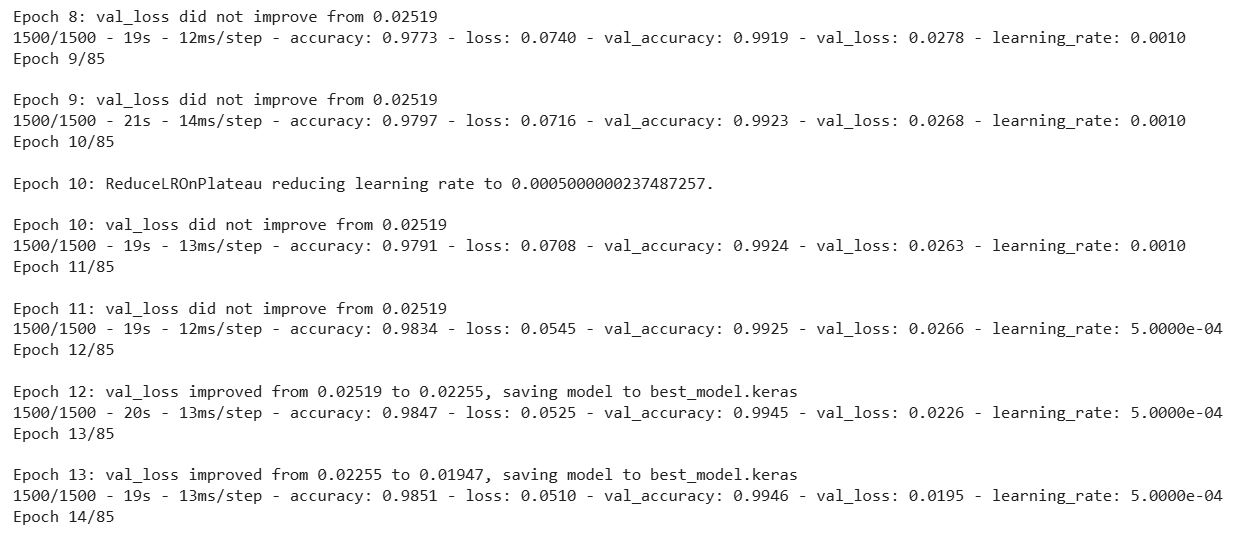
\includegraphics[width=0.7\textwidth]{imgs/explain-callbacks.JPG}
	\caption{Ejemplo del funcionamiento de los callbacks}
	\label{fig:explain-callbacks}
\end{figure}

\subsection{Implementación}

El código implementa las siguientes etapas para el entrenamiento y evaluación del modelo:

\begin{enumerate}
	\item \textbf{División y aumento de datos}:
	\begin{itemize}
		\item Los datos de entrenamiento se dividen en conjuntos de entrenamiento y validación usando \texttt{train\_test\_split}.
		\item El aumento de datos se realiza con \texttt{ImageDataGenerator}, aplicando transformaciones como rotación (10°), desplazamientos (10\%) y zoom (10\%) en los datos de entrenamiento. Para los datos de validación, no se aplica aumento.
	\end{itemize}
	
	\begin{figure}[H]
		\centering
		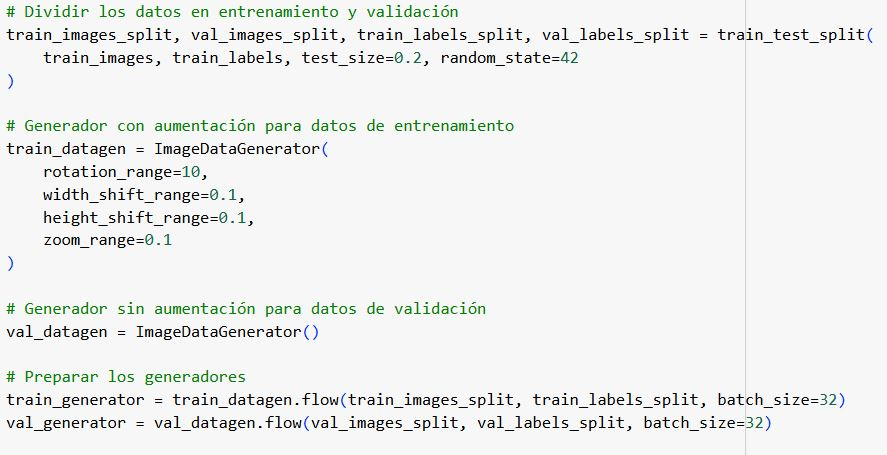
\includegraphics[width=0.7\textwidth]{imgs/model-1-red5.JPG}
		\caption{Modelado de la quinta red neuronal (pt. 1)}
		\label{fig:model-1-red5}
	\end{figure}
	
	\item \textbf{Definición del modelo}:
	\begin{itemize}
		\item La arquitectura del modelo incluye:
		\begin{itemize}
			\item Dos bloques convolutivos con 64 y 128 filtros, kernel (3, 3), y activación \texttt{ReLU}.
			\item Capas de \textit{max-pooling} (2, 2) para reducir dimensionalidad.
			\item Capas de \textit{dropout} para prevenir el sobreajuste.
			\item Una capa densa con 256 unidades y activación \texttt{ReLU}.
			\item Una capa de salida con activación \textit{softmax} para clasificación multiclase.
		\end{itemize}
		\item El modelo se compila usando el optimizador \textit{adam} con tasa de aprendizaje inicial de 0.001, y pérdida \texttt{categorical\_crossentropy}.
	\end{itemize}
	
	\begin{figure}[H]
		\centering
		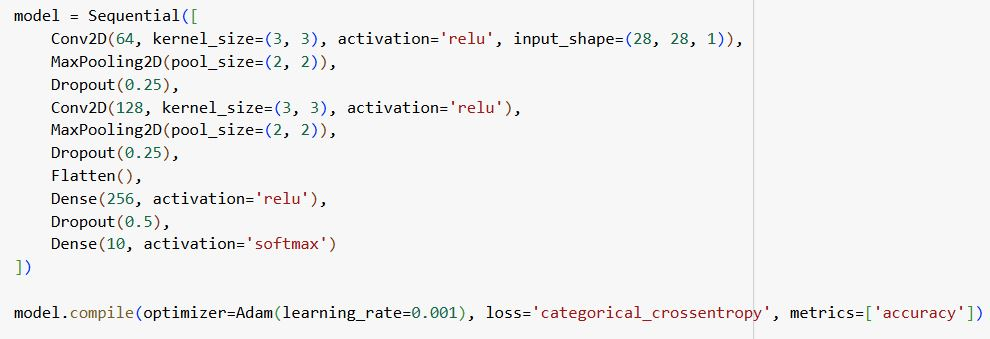
\includegraphics[width=0.7\textwidth]{imgs/model-2-red5.JPG}
		\caption{Modelado de la quinta red neuronal (pt. 2)}
		\label{fig:model-2-red5}
	\end{figure}
	
	\item \textbf{Entrenamiento del modelo}:
	\begin{itemize}
		\item El entrenamiento utiliza generadores para los datos de entrenamiento y validación, aplicando aumento de datos en los primeros.
		\item Se configuran \textit{callbacks} como \texttt{EarlyStopping}, \texttt{ReduceLROnPlateau}, y \texttt{ModelCheckpoint} para mejorar la eficiencia del entrenamiento.
		\item El modelo es entrenado durante un máximo de 85 épocas (no suele alcanzar este límite, ya que se detiene normalmente en la época 40-50), con un tamaño de lote de 32.
	\end{itemize}
	
	\begin{figure}[H]
		\centering
		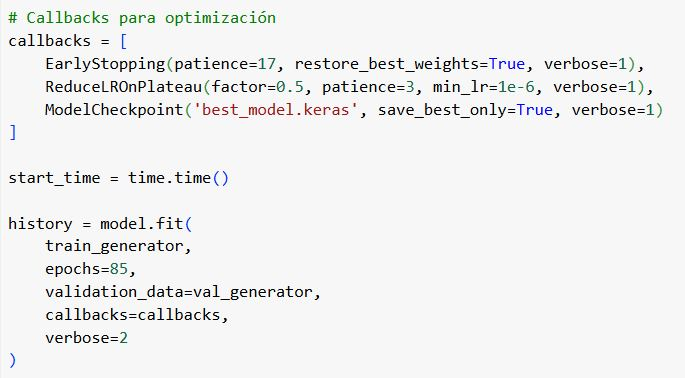
\includegraphics[width=0.7\textwidth]{imgs/model-3-red5.JPG}
		\caption{Modelado de la quinta red neuronal (pt. 3)}
		\label{fig:model-3-red5}
	\end{figure}
\end{enumerate}

\subsection{Análisis de resultados}

\begin{figure}[H]
	\centering
	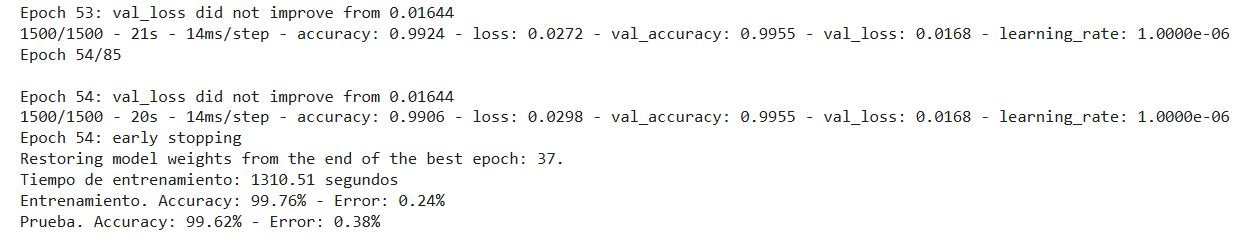
\includegraphics[width=0.7\textwidth]{imgs/results-red5.JPG}
	\caption{Resultados de la cuarta red neuronal}
	\label{fig:results-red5}
\end{figure}

Esta red mejorada, que incluye técnicas avanzadas como aumento de datos, \textit{dropout}, y \textit{callbacks}, logró los mejores resultados entre todas las evaluadas. Con el mínimo error de prueba alcanzado hasta el momento (solo 0.38\%, pudiendo variar entre 0.38-0.41\% de una ejecución a otra) este modelo destaca por su capacidad de generalización y resistencia al sobreajuste.

Aunque su tiempo de entrenamiento es bastante más elevado en comparación con los anteriores, demuestra cómo la integración de estrategias avanzadas puede maximizar el rendimiento, superando incluso a la NN-3 en precisión y estabilidad.

\newpage
\section{Red neuronal combinada NN-4+5 (NN-6)}

Dado que no se alcanzó el 0.3\% de error de prueba deseado, se intentó desarrollar una red neuronal que combinara el enfoque de la NN-4 y la NN-5 implementación.

\subsection{Fundamentos teóricos}

Este modelo combina dos componentes clave: un autoencoder convolucional para extracción de características y una red convolucional supervisada para clasificación. Las etapas y técnicas involucradas son:

\begin{itemize}
	\item \textbf{Autoencoder convolucional}:
	\begin{itemize}
		\item El autoencoder tiene un \textit{codificador} que utiliza capas convolutivas (\texttt{Conv2D}) con activación \texttt{ReLU} y capas de \textit{max-pooling} (\texttt{MaxPooling2D}) para reducir dimensionalidad espacial y capturar características relevantes. La representación comprimida se almacena en la variable \textit{encoded}.
		\item El \textit{decodificador} reconstruye la entrada a partir de la representación comprimida usando capas de \textit{upsampling} (\texttt{UpSampling2D}) y convolutivas, con una capa final que utiliza activación \textit{sigmoid} para producir una salida en el rango [0, 1].
	\end{itemize}
	
	\item \textbf{Red convolucional supervisada}:
	\begin{itemize}
		\item Las características comprimidas extraídas por el autoencoder son utilizadas como entrada para la red convolucional supervisada, que incluye:
		\begin{itemize}
			\item Capas convolutivas (\texttt{Conv2D}) y de \textit{max-pooling}, que procesan las características comprimidas.
			\item Capas de \textit{dropout} (\texttt{Dropout}) con tasas del 25\% y 50\% para reducir el sobreajuste.
			\item Capas densas para integrar las características y realizar la clasificación final mediante una capa con activación \textit{softmax}.
		\end{itemize}
	\end{itemize}
	
	\item \textbf{Optimización y regularización}:
	\begin{itemize}
		\item La red convolucional se optimiza con el algoritmo \textit{adam}, que ajusta dinámicamente la tasa de aprendizaje y combina gradientes adaptativos con momentos para lograr convergencia rápida.
		\item El uso de \textit{callbacks} como \texttt{EarlyStopping}, \texttt{ReduceLROnPlateau}, y \texttt{ModelCheckpoint} permite mejorar la eficiencia del entrenamiento, evitar sobreajuste y ajustar la tasa de aprendizaje de manera dinámica.
	\end{itemize}
\end{itemize}

El enfoque completo aprovecha las capacidades de los autoencoders para extraer representaciones comprimidas útiles y mejora el desempeño del modelo supervisado mediante una mejor inicialización de datos y regularización.


\subsection{Implementación}

El modelo implementado sigue los siguientes pasos:

\begin{enumerate}
	\item \textbf{Creación y entrenamiento del autoencoder}:
	\begin{itemize}
		\item Se define un autoencoder con un \textit{codificador} compuesto por dos capas \texttt{Conv2D} (32 y 64 filtros) y dos capas \texttt{MaxPooling2D} para comprimir las características de entrada.
		\item El \textit{decodificador} utiliza capas \texttt{Conv2D} y \texttt{UpSampling2D} para reconstruir las imágenes originales.
		\item El modelo se entrena durante 10 épocas, utilizando el optimizador \textit{adam} y la pérdida \texttt{binary\_crossentropy}, con un tamaño de lote de 256 y una validación del 20\%.
	\end{itemize}
	
	\begin{figure}[H]
		\centering
		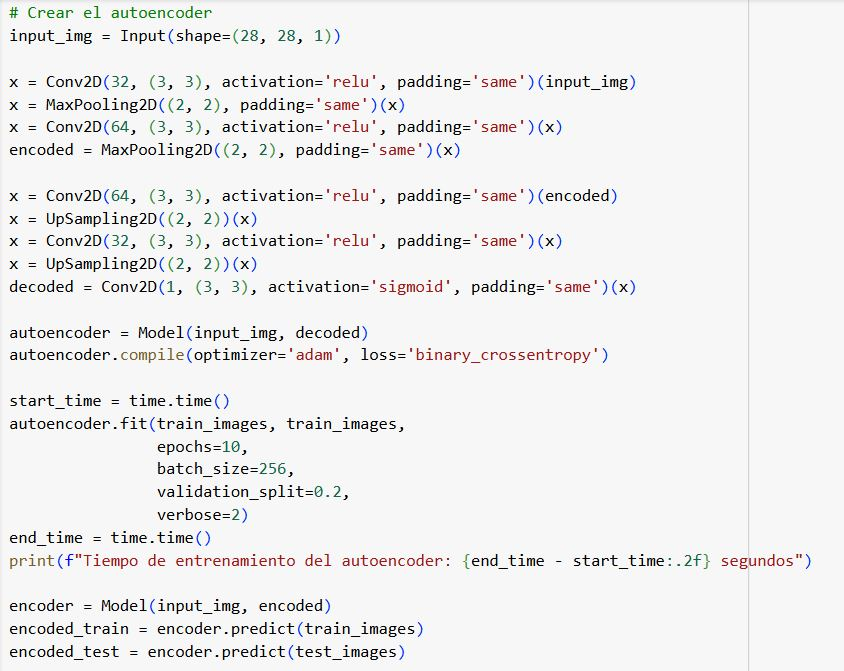
\includegraphics[width=0.7\textwidth]{imgs/model-1-red6.JPG}
		\caption{Modelado de la sexta red neuronal (pt. 1)}
		\label{fig:model-1-red6}
	\end{figure}
	
	\item \textbf{Generación de conjuntos de entrenamiento y validación}:
	\begin{itemize}
		\item Se utilizan los datos comprimidos generados por el codificador para dividirlos en conjuntos de entrenamiento y validación mediante \texttt{train\_test\_split}.
		\item Se aplica aumento de datos (\texttt{ImageDataGenerator}) a los datos de entrenamiento mediante rotaciones, desplazamientos y zoom, mientras que los datos de validación no se modifican.
	\end{itemize}
	
	\item \textbf{Creación y entrenamiento del modelo supervisado}:
	\begin{itemize}
		\item La red convolucional supervisada incluye dos bloques convolutivos (64 y 128 filtros), seguidos de capas de \textit{max-pooling} y \textit{dropout}.
		\item Se utiliza una capa densa con 256 neuronas y activación \texttt{ReLU}, seguida de una capa de salida con activación \texttt{softmax}.
		\item El modelo es compilado usando el optimizador \textit{adam} con tasa de aprendizaje inicial 0.001, y pérdida \texttt{categorical\_crossentropy}.
	\end{itemize}
	
	\begin{figure}[H]
		\centering
		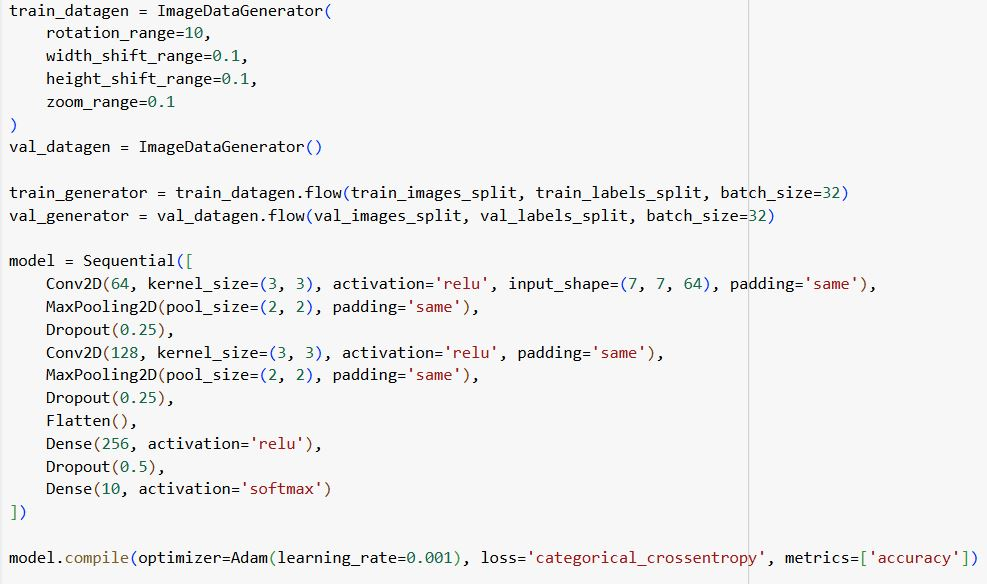
\includegraphics[width=0.7\textwidth]{imgs/model-2-red6.JPG}
		\caption{Modelado de la sexta red neuronal (pt. 2)}
		\label{fig:model-2-red6}
	\end{figure}
	
	\item \textbf{Configuración de \textit{callbacks} y entrenamiento}:
	\begin{itemize}
		\item \texttt{EarlyStopping} detiene el entrenamiento si la métrica de validación no mejora tras 7 épocas consecutivas.
		\item \texttt{ReduceLROnPlateau} ajusta dinámicamente la tasa de aprendizaje cuando se alcanza un \textit{plateau} en el desempeño.
		\item \texttt{ModelCheckpoint} guarda el mejor modelo basado en la pérdida de validación.
		\item El entrenamiento se realiza durante un máximo de 50 épocas, utilizando generadores para los datos de entrenamiento y validación.
	\end{itemize}
	
	\begin{figure}[H]
		\centering
		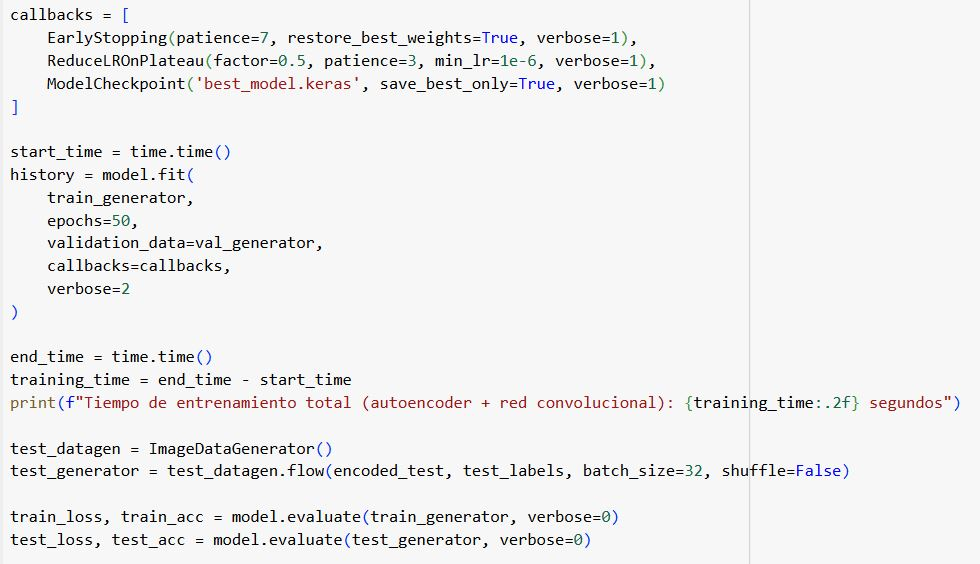
\includegraphics[width=0.7\textwidth]{imgs/model-3-red6.JPG}
		\caption{Modelado de la sexta red neuronal (pt. 3)}
		\label{fig:model-3-red6}
	\end{figure}
\end{enumerate}


\subsection{Análisis de resultados}

\begin{figure}[H]
	\centering
	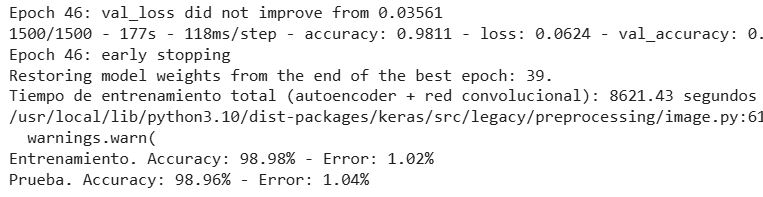
\includegraphics[width=0.7\textwidth]{imgs/results-red6.JPG}
	\caption{Resultados de la sexta red neuronal}
	\label{fig:results-red6}
\end{figure}

Aunque se consiguió reducir el error de la NN-4, no mostró una mejora con respecto a la NN-5, es más, los resultados obtenidos eran similares a los de NN-3. Esto, sumado al hecho de que llegó a tardar 2h40, llevó a la conclusión de que este enfoque combinado no era el más adecuado.

\newpage
\section{Refinamiento de la NN-5 (NN-7)}

Como último intento para reducir el error de prueba, se optó por tratar de mejorar la NN-5 (la CNN mejorada), ya que fue la que mejores resultados obtuvo de las implementadas hasta ahora.

\subsection{Fundamentos teóricos}

Esta red neuronal es una versión mejorada de la arquitectura de la NN-5, donde se han agregado técnicas avanzadas de regularización y normalización para optimizar el rendimiento del modelo. Los aspectos teóricos clave de estas mejoras incluyen:

\begin{itemize}
	\item \textbf{Batch normalization}:
	\begin{itemize}
		\item Se incorpora después de cada capa convolutiva (\texttt{Conv2D}). La normalización por lotes reescala las activaciones para que tengan media 0 y varianza 1 durante el entrenamiento. Esto acelera la convergencia, estabiliza el aprendizaje y reduce la sensibilidad a la inicialización de pesos \parencite{ioffe2015batchnorm}.
	\end{itemize}
	
	\item \textbf{Regularización L2 en la capa densa}:
	\begin{itemize}
		\item La regularización L2 penaliza pesos grandes en el modelo, reduciendo el sobreajuste. Esto se implementa en la capa densa con la función de penalización \texttt{regularizers.l2
		(0.01)}, donde el término de regularización se añade a la función de pérdida \parencite{goodfellow2016deep}.
	\end{itemize}
	
	\item \textbf{Global Average Pooling}:
	\begin{itemize}
		\item En lugar de \textit{max-pooling}, la última capa convolutiva utiliza \texttt{GlobalAveragePooling2D}, que reduce cada mapa de características a un único valor promedio. Esto minimiza la cantidad de parámetros en la transición a las capas densas, reduciendo el riesgo de sobreajuste \parencite{lin2013network}.
	\end{itemize}
	
	\item \textbf{Optimización}:
	\begin{itemize}
		\item Se utiliza el optimizador \textit{adam} con una tasa de aprendizaje ajustada a 0.0005, lo que permite actualizaciones más precisas en la etapa final del entrenamiento. La pérdida es \texttt{categorical\_crossentropy}, adecuada para tareas de clasificación multiclase.
	\end{itemize}
	
	\item \textbf{Callbacks}:
	\begin{itemize}
		\item Se ha hecho un pequeño ajuste para que la paciencia del EarlyStopping sea un poco menor (10 en lugar de 17), en un intento de acelerar el entrenamiento del modelo. 
	\end{itemize}
\end{itemize}

\subsection{Implementación}

Esta red neuronal mejora la arquitectura de la NN-5 mediante la adición de nuevas técnicas y cambios clave:

\begin{enumerate}
	\item \textbf{Capa convolutiva y normalización por lotes}:
	\begin{itemize}
		\item Se utilizan tres bloques convolutivos con 64, 128 y 256 filtros, kernel (3, 3), y activación \texttt{ReLU}.
		\item Después de cada convolución, se añade una capa \texttt{BatchNormalization()} para estabilizar y acelerar el entrenamiento.
		\item Cada bloque incluye también \texttt{MaxPooling2D} para reducción espacial y \texttt{Dropout} con tasas de 20\%, 30\% y 40\% respectivamente.
	\end{itemize}
	
	\item \textbf{Capa de \textit{Global Average Pooling}}:
	\begin{itemize}
		\item En lugar de aplicar \textit{flattening} directamente los mapas de características, se utiliza \texttt{GlobalAveragePooling2D()}, que reduce cada mapa de características a un único valor promedio, disminuyendo la dimensionalidad de manera eficiente.
	\end{itemize}
	
	\item \textbf{Capa densa regularizada}:
	\begin{itemize}
		\item Una capa densa con 256 neuronas y activación \texttt{ReLU}, que incluye regularización L2 con un coeficiente de 0.01.
		\item Se añade una capa \texttt{Dropout(0.4)} antes de la capa de salida.
	\end{itemize}
	
	\item \textbf{Capa de salida}:
	\begin{itemize}
		\item La capa final es una capa densa con 10 neuronas y activación \textit{softmax} para la clasificación multiclase.
	\end{itemize}
	
	\item \textbf{Compilación y optimización}:
	\begin{itemize}
		\item El modelo es compilado con el optimizador \textit{adam}, ajustado con una tasa de aprendizaje de 0.0005, y pérdida \texttt{categorical\_crossentropy}.
	\end{itemize}
\end{enumerate}

\begin{figure}[H]
	\centering
	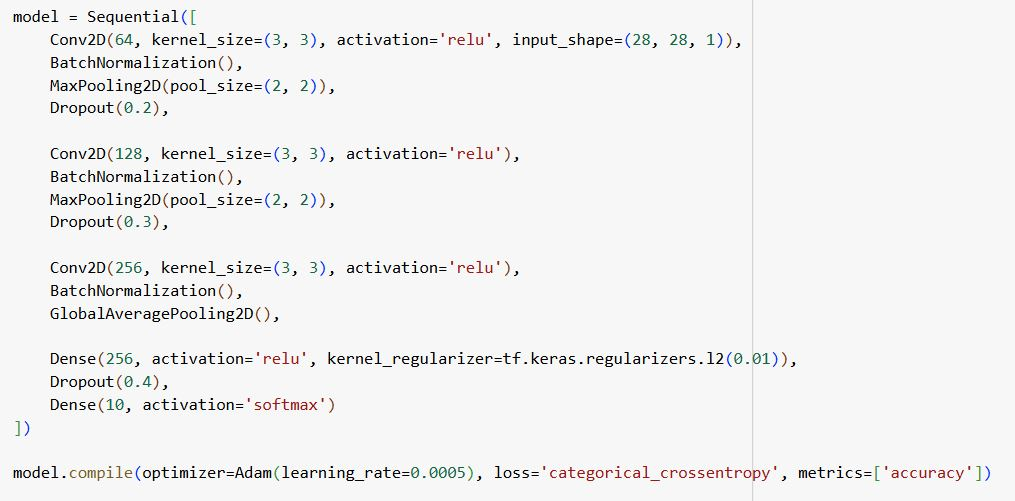
\includegraphics[width=0.7\textwidth]{imgs/model-red7.JPG}
	\caption{Modelado de la séptima red neuronal}
	\label{fig:model-red7}
\end{figure}

\subsection{Análisis de resultados}

\begin{figure}[H]
	\centering
	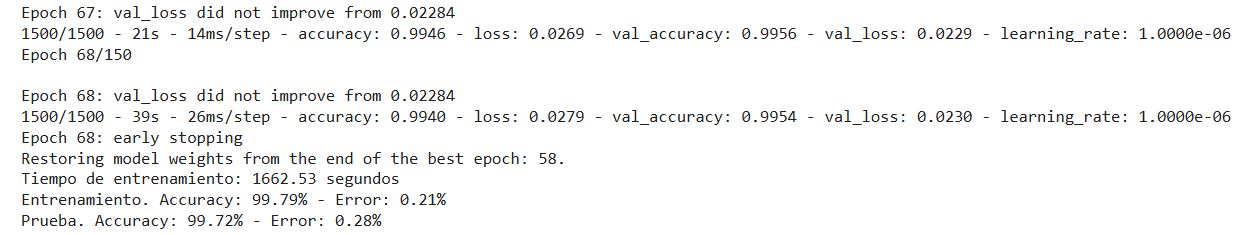
\includegraphics[width=0.7\textwidth]{imgs/results-red7.JPG}
	\caption{Resultados de la séptima red neuronal}
	\label{fig:results-red7}
\end{figure}

Finalmente, se ha logrado mejorar la precisión, obteniendo un error sobre el conjunto de prueba del 0.28\%, gracias a las mejoras implementadas sobre la arquitectura de la NN-5. Por tanto, se ha alcanzado el objetivo de llegar a un porcentaje de error menor o igual que el 0.3\%, mediante la NN-7, que es una nueva versión mejorada de la CNN.
